\newcommand{\drawU}[1]{
		\draw[thick] (#1.north east) -- (#1.north west) --
			  (#1.south west) -- (#1.south east);
}

\newcommand{\legendforblocks}[0]{%
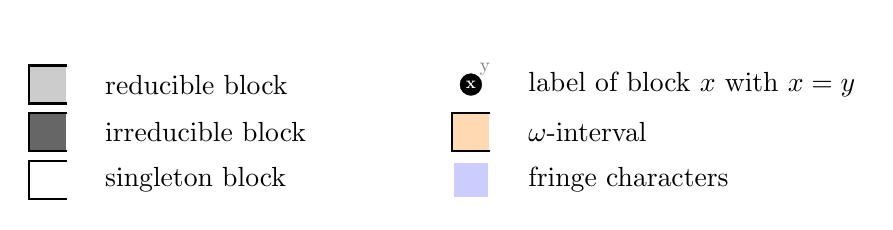
\begin{tikzpicture}[legendbox/.style={inner sep=1.5ex,draw=black,thick}]
	\begin{scope}[node distance=4ex]
		\node[] (leg0) at (0,0) {};
		\node[below of=leg0, inner sep=1.5ex,st_reducible,alias=leg1] 
			 (reduciblebox) {};
		\drawU{reduciblebox}
		\node[right of=reduciblebox, right] {reducible block};

		\node[below of=leg1, inner sep=1.5ex,st_irreducible,alias=leg2] (irreduciblebox) {};
		\drawU{irreduciblebox}
		\node[right of=irreduciblebox, right] (irrlabel) 
		     {irreducible block};
		\node[below of=leg2, inner sep=1.5ex,st_singleton,alias=leg3] (singletonbox) {};
		\drawU{singletonbox}
		\node[right of=singletonbox, right] {singleton block};

		\coordinate[xshift=12ex] (block_label_pos) at (leg1 -| irrlabel.east);
	%	\node[shape=circle,draw=blue,inner sep=0.2mm] at (leg1) {};
	%	\node[shape=circle,draw=green,inner sep=0.2mm] at (irrlabel.east) {};
	%	\node[shape=circle,draw=red,inner sep=0.2mm] at (block_label_pos) {};
	%	\draw[st_]
		\node[st_block_fwd_id_label, right] (block_label) at 
			  (block_label_pos) {x}; 
		\node[st_block_bwd_id_label,node distance=0ex] (block_bwd_id_label) at (block_label.north east) {y};
%		\node[shape=circle, draw=red,inner sep=0.2mm] at (block_label.north east) {};
		\node[right of=block_label, right]{label of block $x$ with $\bwdid{x}=y$};

		\node[below of=block_label, inner sep=1.5ex,st_interval,alias=leg4] 
			 (omega interval box) {};
		\drawU{omega interval box}
		\node[right of=omega interval box, right] {$\omega$-interval};

		\node[below of=leg4, inner sep=1.5ex, st_fringe,alias=leg5] (fringe box) {};
		\node[right of=leg5, right] {fringe characters};
	\end{scope}
\end{tikzpicture}%
}

\newcommand{\getdeltax}[1]{
	\coordinate (deltax) at ($#1*(text0.west)-#1*(text0.east)+#1*2*(\pgflinewidth,0)$);
}

% \param number of the start of the interval
% \param number of the end of the interval
% \param depth of the interval
% \param name of the column
% \param style options
\newcommand{\markintervalleft}[5]{%
\begin{tikzpicture}[overlay, remember picture,font=\tt,show background rectangle]
	\getdeltax{#3}
	\draw[#5] (#4#1.north west) ++ ($(0,0)-(deltax)$) -- ++ (deltax) 
	           -- (#4#2.south west) -- ++ ($(0,0)-(deltax)$);
\end{tikzpicture}%
}

% \param number of the start of the interval
% \param number of the end of the interval
% \param depth of the interval
% \param name of the column
% \param style options
\newcommand{\markintervalright}[5]{%
\begin{tikzpicture}[overlay,remember picture, font=\tt, st_mark_interval_right]
	\getdeltax{#3}
	\draw[#5] (#4#1.north east) -- ++ (deltax) -- 
	          ($(#4#2.south east)+ (deltax)$) -- 
			  ++ ($(0,0)-(deltax)$);
	\draw (#4#1.north east) -- ++ (deltax) -- 
	          ($(#4#2.south east)+ (deltax)$) -- 
			  ++ ($(0,0)-(deltax)$);
\end{tikzpicture}%
}

% \param index in the suffix array [0..n-1]
% \param depth of the fringe [0..n-1]
% \param length of the fringe [1..n-1]
% \param style
\newcommand{\markfringe}[4]{%
\begin{tikzpicture}[overlay,remember picture, font=\tt]
	\getdeltax{1}
	\draw[#4] ($(text#1.north west)-#2*(deltax)-#2*(\pgflinewidth,0)$) 
			  rectangle ($(text#1.south west)-#2*(deltax)-#3*(deltax)-#2*(\pgflinewidth,0)$);
\end{tikzpicture}%
}

% \param indexes in the suffix array [0..n-1] as array e.g. {0,1,2,3,8}
% \param depth of the fringe [0..n-1] as array e.g. {3,4,5,4,3}
% \param length of the fringe [1..n-1]
% \param style
\newcommand{\markfixedfringes}[4]{
	\foreach \idx [count=\i from 0] in #1{
		\pgfmathparse{array(#2,\i)}\let\fringedepth\pgfmathresult
		\markfringe{\idx}{\fringedepth}{#3}{#4}	
	}
}


% \param indexes in the suffix array [0..n-1] as array e.g. {0,1,2,3,8}
% \param depth of the fringe [0..n-1] as array e.g. {3,4,5,4,3}
% \param length of the fringe [1..n-1] as array e.g. {1,2,3,1,2}
% \param style
\newcommand{\markvarfringes}[4]{
	\foreach \idx [count=\i from 0] in #1{
		\pgfmathparse{array(#2,\i)}\let\fringedepth\pgfmathresult
		\pgfmathparse{array(#3,\i)}\let\fringelen\pgfmathresult
		\markfringe{\idx}{\fringedepth}{\fringelen}{#4}	
	}
}

% \param number of the start of the interval
% \param number of the end of the interval
% \param name of the column
% \param name of the anchor
\newcommand{\intervalanchor}[4]{
	\tikz[overlay,remember picture] \coordinate (#4) at ($(#3#1.east)!0.5!(#3#2.east)$);
	\tikz[overlay,remember picture] \coordinate (#4_start) at (#3#1.north east);
	\tikz[overlay,remember picture] \coordinate (#4_start_east) at (#3#1.north east);
	\tikz[overlay,remember picture] \coordinate (#4_end) at (#3#2.south east);
}

% \param source block id
% \param destination block id
% \param style
\newcommand{\intervaledge}[3]{%
	\begin{tikzpicture}[overlay, remember picture, st_block_info]
		\coordinate (block1_coord) at ($(block#1)-(3.5ex,0.5ex)$);
		\coordinate (block2_coord) at ($(block#2)-(3.5ex,-0.5ex)$);
		\ifnum #1 > #2
			\draw[st_interval_edge, #3] (block1_coord) to[bend left=30] (block2_coord);
		\else
			\ifnum #1 < #2
				\draw[st_interval_edge, #3] (block1_coord) to[bend right=30] (block2_coord);
			\else % #1 == #2
				\draw[fill=black] ($(block1_coord)-(0.5ex,-0.5ex)$) circle (2pt);
			\fi	
		\fi
	\end{tikzpicture}%
}
% \param source block id 
% \param destination block id 
% \param delta
\newcommand{\intervaledgereducible}[3]{%
	\begin{tikzpicture}[overlay, remember picture, st_block_info]
		\coordinate (len#1) at ($(block#1_end)-(block#1_start)$);
		\coordinate (line_height) at ($(i0.north)-(i1.north)$);
		\coordinate (block1_coord2) at ($(block#1)-(3.5ex,0ex)$);
		\coordinate (block2_coord2) at ($(block#2_start)-(3.5ex,0ex)-#3*(line_height)+1/2.0*(len#1)$);
		\ifnum #1 > #2
			\draw[st_reducible_edge] (block1_coord2) to[bend left=30] (block2_coord2);
		\else
			\ifnum #1 < #2
				\draw[st_reducible_edge] (block1_coord2) to[bend right=30] (block2_coord2);
			\else % #1 == #2
				\draw[fill=black] ($(block1_coord2)-(0.5ex,-0.5ex)$) circle (2pt);
			\fi	
		\fi	
	\end{tikzpicture}%
}
% \param block id
% \param delta (x-offset in the final irreducible block)
% \param times (to iterate to get to a irreducible block)
% \param dest_block (pointer to the corresponding irreducible block)	
\newcommand{\blockinfo}[5]{%
\begin{tikzpicture}[overlay, remember picture, st_block_info]
	\ifnum #1 = #4
		% do nothing for irreducible and singleton intervals
	\else
		% draw block info for reducible blocks
		\node[below right,scale=0.7, align=left] (block_info#1) at ($(block#1_start_east)$) 
		 {$\deltax=#2$\ \\$\deltad=#3$};
	\fi
	% draw block id label
	\node[right, st_block_fwd_id_label,xshift=10ex] (block_fwd_id#1) 
	      at ($(block#1_start_east)$) {#1};
	\draw[st_line_to_block_fwd_id_label] (block#1_start_east) -- (block_fwd_id#1);
	% TODO 
	\node[st_block_bwd_id_label] (bwd_block_fwd_id#1) at (block_fwd_id#1.north east) {#5};
\end{tikzpicture}%
}
% \param block id  
% \param block header is an array of the form {bwd_id, delta_x, delta_d}
\newcommand{\externalblockheader}[2]{%
\begin{tikzpicture}[overlay, remember picture, st_block_info,node distance=0ex, inner sep=0.2mm]
	\foreach \item [count=\i from 1, count=\j from 0] in #2{
		\pgfmathparse{#2[\j][0]}\let\ID\pgfmathresult
		\pgfmathparse{#2[\j][1]}\let\DELTAX\pgfmathresult
		\pgfmathparse{#2[\j][2]}\let\DELTAD\pgfmathresult
%		\typeout{i=\i j=\j item=\item}	
		\ifnum \j > 0
			\node[below left, st_block_header] 
			     (block_header_#1_\i) at 
				 (block_header_#1_\j.south east)
				 {$(\ID,\DELTAX,\DELTAD)$};
		\else
			\node[below left, st_block_header] (block_header_#1_\i) at (block_fwd_id#1.south west) 
			     {$(\ID,\DELTAX,\DELTAD)$};

		\fi	
	}
\end{tikzpicture}%
}

\newcommand{\drawheaderfwd}[0]{%
\begin{tikzpicture}[remember picture, overlay, every node/.style={inner sep=0cm}]
	\coordinate[st_fwd_index_header] (yHeader) at (y0);
	\node[st_elem_i] at (i |- yHeader) {$i$};
	\node[st_elem_sa] at (sa |- yHeader) {$\SUF[i]$};
	\node[st_elem_lcp] at (lcp |- yHeader) {$\LCP[i]$};
	\node[st_elem_bwt] at (bwt |- yHeader) {$\BWT[i]$};
	\node[st_elem_fwdbf] at (fwdbf |- yHeader) {$\fwdbf[i]$};
	\coordinate (text_label_pos) at (text0.west |- yHeader);
	\node[st_elem_text] at (text_label_pos) {$\TEXT[\SUF[i]..n]$};
%	\node[shape=circle,draw=red,inner sep=0.2mm] at (fwdbf |- yHeader) {};
%	\node[shape=circle,draw=red,inner sep=0.2mm] at (text_label_pos) {};
\end{tikzpicture}%
}
\newcommand{\drawheaderbwd}[0]{%
\begin{tikzpicture}[remember picture, overlay, every node/.style={inner sep=0cm}]
	\coordinate[st_bwd_index_header] (yHeader) at (y0);
	\node[st_elem_i] at (i |- yHeader) {$i$};
%	\node[st_elem_lcp] at (lcp |- yHeader) {$\LCP[i]$};
	\node[st_elem_bwt] at (bwt |- yHeader) {$\BWT^{\TEXT^{r}}[i]$};
	\node[st_elem_bwdbl] at (bwdbl |- yHeader) {$\bwdbl[i]$};
	\node[st_elem_bwdbf] at (bwdbf |- yHeader) {$\bwdbf[i]$};
	\coordinate (text_label_pos) at (text0.west |- yHeader);
	\node[st_elem_text] at (text_label_pos) {$\TEXT^{r}[\SUF[i]..n]$};
\end{tikzpicture}%
}
% Note: the macro \fwdBlocksInBwd should contain a pgf array
% with the data for this command
\newcommand{\markFwdBlocksInBwdIndex}[0]{
	\foreach \block [count=\bwdId from 0] in \fwdBlocksInBwd{
		\pgfmathparse{int(array(\block,0))}\let\bwdlb\pgfmathresult
		\pgfmathparse{int(array(\block,1)-1)}\let\bwdrb\pgfmathresult
		\pgfmathparse{int(array(\block,2))}\let\fwddepth\pgfmathresult
		\pgfmathparse{int(array(\block,3))}\let\fwdblockid\pgfmathresult
		\markintervalleft{\bwdlb}{\bwdrb}{\fwddepth}{text}{st_interval}%
		\begin{tikzpicture}[overlay, remember picture]%
			\node[st_block_fwd_id_label,opacity=0] (tmp) at (0,0) {\fwdblockid};
			\coordinate (dim) at ($(tmp.east)-(tmp.west)$);
			\coordinate (fwd_block_fwd_id_\bwdlb_\fwddepth_pos) at % 
			  			($(text\bwdlb.north east)+\fwddepth*(dim)$);
			\draw[st_line_to_block_fwd_id_label] %
			     (text\bwdlb.north west) -- %
				 (fwd_block_fwd_id_\bwdlb_\fwddepth_pos);
			\node[st_block_fwd_id_label, below] (fwd_block_fwd_id_\bwdlb_\fwddepth) %
			  at (fwd_block_fwd_id_\bwdlb_\fwddepth_pos) {\fwdblockid};
			\node[shape=circle,draw=black,inner sep=0.2mm,fill=black] at 
				(fwd_block_fwd_id_\bwdlb_\fwddepth_pos) {};

			\node[st_block_bwd_id_label] at (fwd_block_fwd_id_\bwdlb_\fwddepth_pos) {\bwdId};
		\end{tikzpicture}%
	}
}
\newcommand{\bwdIndexLayout}[0]{
\tikzstyle{st_i} = [xshift=-0.4cm]\tikzstyle{st_elem_i} = [left]
\tikzstyle{st_lcp} = [xshift=2.3cm]\tikzstyle{st_elem_lcp} = [left,opacity=0]
\tikzstyle{st_bwt} = [xshift=1cm] \tikzstyle{st_elem_bwt} = [left]
\tikzstyle{st_bwdbl} = [xshift=2cm] \tikzstyle{st_elem_bwdbl} = [left]
\tikzstyle{st_bwdbf} = [xshift=3cm] \tikzstyle{st_elem_bwdbf} = [left]
\tikzstyle{st_text} = [xshift=3.4cm] \tikzstyle{st_elem_text} = [right]
}
% depends on the existence of arrays \bwdBlArray and \bwdBWTArray
\newcommand{\printBlAndCBWT}[0]{%
\begin{tikzpicture}[remember picture]
	\begin{scope}[node distance=1.5ex,font=\tt]
		\coordinate (bwdBl0) at (0,0);
		\coordinate (bwdBWT0) at (0,-3ex);
		\node[left=-1.5ex of bwdBl0] {$\bwdbl =\ $};
		\node[left=-1.5ex of bwdBWT0] {$\cL =\ $};
		\foreach \x [count=\i from 0, count=\j from 1] in \bwdBlArray{
			\node[right, right of=bwdBl\i] (bwdBl\j) {\x};
			\ifnum \x = 1
				\pgfmathparse{{\bwdBWTArray}[\i]}\let\bwt\pgfmathresult
				\node[text height=2ex, text depth=1ex] at (bwdBl\j |- bwdBWT0) {\bwt};
			\fi	
		}
	\end{scope}
\end{tikzpicture}%
}
\newcounter{minPosCnt}
%depends on the existence of arrays \bmArray and \minDepth
\newcommand{\printBmAndMinDepth}[0]{%
\begin{tikzpicture}[remember picture]
	\begin{scope}[node distance=1.5ex,font=\tt]
	\setcounter{minPosCnt}{0}
		\coordinate (bwdbm0) at (0,0);
		\coordinate (minDepth0) at (0,-3ex);
		\coordinate (XY) at (bwdbm0 |- minDepth0);
		\node[left=-1.5ex of bwdbm0] {$\bwdbm =\ $};
		\node[left=-1.5ex of XY] {$\bwdmindepth =\ $};
		\foreach \x [count=\i from 0, count=\j from 1] in \bmArray{
			\node[right, right of=bwdbm\i] (bwdbm\j) {\x};
			\ifnum \i > 0 
				\pgfmathparse{ int( {\bmArray}[\i] && ({\bmArray}[int(\i-1)] == 0) }\let\ENTRIES\pgfmathresult
				\ifnum \ENTRIES = 1 
					\pgfmathparse{{\minDepthArray}[int(\theminPosCnt)]}\let\minDepth\pgfmathresult
					\node[text height=2ex, text depth=1ex] at (bwdbm\j |- minDepth0) {\minDepth};
					\addtocounter{minPosCnt}{1}
				\fi	
			\fi	
		}
	\end{scope}
\end{tikzpicture}%
}
%depends on the existence of arrays \bmArray and \minDepth
\newcommand{\printFac}[0]{%
\begin{tikzpicture}[remember picture]
%	\begin{scope}[node distance=1.5ex,font=\tt]
	\begin{scope}[text height=2ex, text depth=1ex]
%		\coordinate (facArray0) at (0,0);
%		\node[left=-1.5ex of facArray0] {$FZ =\ $\phantom{,}};
%		\foreach \x [count=\i from 0, count=\j from 1] in \facArray{
%			\node[node distance=0ex, right, right=of facArray\i,inner xsep=0] (facArray\j) { %
%				\ifnum \i > 0
%					,
%				\else
%					\phantom{,}	
%				\fi	
%				\x %
%			};
%		}
		\setcounter{minPosCnt}{0}
		\coordinate (FwdText0) at (0,-2);
		\coordinate (Factor0) at (0,-1.2);
		\node[left=-1.5ex of FwdText0] {Expansion \quad\phantom{,}};
		\node[left=-1.5ex of Factor0] {Factors $\TEXT'$ \quad\phantom{,}};
		\foreach \x [count=\i from 0, count=\j from 1] in \facLen{
			\pgfmathparse{\theminPosCnt}\let\start\pgfmathresult
			\pgfmathparse{int(\theminPosCnt+1)}\let\startpp\pgfmathresult
			\pgfmathparse{int(\theminPosCnt+\x-1)}\let\end\pgfmathresult
			\node[node distance=0, right=of FwdText\i, inner sep=1pt] (FwdText\j){%
	%			\foreach \y [count=\i from \start, count=\j from \startpp] in {\start,...,\end} {
				\foreach \y in{\start,...,\end}{ %
					\pgfmathparse{{\FwdText}[\y]}\let\FwdLetter\pgfmathresult%
	%				\node[text height=2ex, text depth=1ex, node distance=0, right=of FwdText\i] (FwdText\j){\FwdLetter};
					{\tt \FwdLetter}%
				}%
			};
			\draw[gray] 
				       ($(FwdText\j.north west)+(1pt,-2pt)$) 
				    -- ($(FwdText\j.north west)+(1pt,0)$) 
				    -- ($(FwdText\j.north east)-(1pt,0)$)
				    -- ($(FwdText\j.north east)-(1pt,2pt)$);
			\pgfmathparse{{\facArray}[\i]}\let\bwdFactor\pgfmathresult
			\node[node distance=1pt, right=of Factor\i,color=gray,font=\small, inner sep=1pt] (Factor\j) {\bwdFactor};
			\draw[color=gray]  ($(Factor\j.south)+(0,4pt)$) -- (FwdText\j.north);  
			\addtocounter{minPosCnt}{\x}
		}
	\end{scope}
\end{tikzpicture}%
}

\tikzstyle{st_block_info} = []
\tikzstyle{st_block_fwd_id_label} = [shape=circle,scale=0.6,fill=black, draw=white,%
                                 inner sep=0mm, minimum size=5mm, font=\bf, text=white]

\tikzstyle{st_block_bwd_id_label} = [scale=0.7,above right,inner sep=0mm,text=gray] 
\tikzstyle{st_line_to_block_fwd_id_label} = [densely dashed]
\tikzstyle{st_mark_interval_right} = []
\tikzstyle{st_i} = [xshift=0cm]
\tikzstyle{st_elem_i} = [left]
\tikzstyle{st_sa} = [xshift=2cm]
\tikzstyle{st_elem_sa} = [left]
\tikzstyle{st_lcp} = [xshift=3.2cm]
\tikzstyle{st_elem_lcp} = [left]
\tikzstyle{st_bwt} = [xshift=4.2cm]
\tikzstyle{st_elem_bwt} = [left]
\tikzstyle{st_fwdbf} = [xshift=5.2cm]
\tikzstyle{st_elem_fwdbf} = [left]
\tikzstyle{st_text} = [xshift=5.6cm]
\tikzstyle{st_elem_text} = [right]
\tikzstyle{st_singleton} = [thick]
\tikzstyle{st_reducible} = [thick, fill=black, opacity=0.2]
\tikzstyle{st_irreducible} = [thick, fill=black, opacity=0.6]
\tikzstyle{st_interval} = [thick, fill=orange, fill opacity=0.3]
\tikzstyle{st_fringe} = [draw=white, fill=blue, fill opacity=0.2]
\tikzstyle{st_right_fringe} = 	%[opacity=0]%
								[st_fringe]
\tikzstyle{st_simple_fringe} = 	[opacity=0]
								%[draw=white, fill=red, fill opacity=0.2]
\tikzstyle{st_left_fringe} = 	%[opacity=0]
								[st_fringe]

\tikzstyle{st_full_fringe} = 	%[opacity=0]
								[st_fringe]




\tikzstyle{st_interval_edge} = [thick, ->, >=stealth]
\tikzstyle{st_reducible_edge} = [very thick, ->, >=stealth']
\tikzstyle{st_fwd_index_header} = [yshift=0.6cm]
\tikzstyle{st_bwd_index_header} = [yshift=0.6cm]
\tikzstyle{st_y} = [node distance=2.6ex]
\tikzstyle{st_block_header} = [text=red, scale=0.7]
